% --------------------------------------------------------------
% This is all preamble stuff that you don't have to worry about.
% Head down to where it says "Start here"
% --------------------------------------------------------------
 
\documentclass[12pt]{article}
 
\usepackage[margin=1in]{geometry} 
\usepackage{amsmath,amsthm,amssymb,mathtools}
\usepackage{float}
\usepackage{graphicx}

\newcommand{\N}{\mathbb{N}}
\newcommand{\Z}{\mathbb{Z}}
\newcommand{\sign}[1]{\text{sign}(#1)}
\newcommand{\abs}[1]{\left| #1 \right|}
\newcommand{\BigO}[1]{\mathcal{O}\left( #1 \right)}
\renewcommand{\Pr}[1]{\text{Pr}[ #1 ]}
 
\newenvironment{theorem}[2][Theorem]{\begin{trivlist}
\item[\hskip \labelsep {\bfseries #1}\hskip \labelsep {\bfseries #2.}]}{\end{trivlist}}
\newenvironment{lemma}[2][Lemma]{\begin{trivlist}
\item[\hskip \labelsep {\bfseries #1}\hskip \labelsep {\bfseries #2.}]}{\end{trivlist}}
\newenvironment{exercise}[2][Exercise]{\begin{trivlist}
\item[\hskip \labelsep {\bfseries #1}\hskip \labelsep {\bfseries #2.}]}{\end{trivlist}}
\newenvironment{problem}[2][Problem]{\begin{trivlist}
\item[\hskip \labelsep {\bfseries #1}\hskip \labelsep {\bfseries #2.}]}{\end{trivlist}}
\newenvironment{question}[2][Question]{\begin{trivlist}
\item[\hskip \labelsep {\bfseries #1}\hskip \labelsep {\bfseries #2.}]}{\end{trivlist}}
\newenvironment{corollary}[2][Corollary]{\begin{trivlist}
\item[\hskip \labelsep {\bfseries #1}\hskip \labelsep {\bfseries #2.}]}{\end{trivlist}}
 
\begin{document}
 
% --------------------------------------------------------------
%                         Start here
% --------------------------------------------------------------
 
\title{Homework 1}%replace X with the appropriate number
\author{Christopher Mertin\\ %replace with your name
CS6966: Theory of Machine Learning} %if necessary, replace with your course title
 
\maketitle

\begin{enumerate}
\item Consider the problem of classifying points in the two-dimensional plane, {\em i.e.}, $\chi = \mathbb{R}^{2}$. Suppose that the (unknown) true label of a point $(x,y)$ is given by $\sign{x}$ (we define $\sign{0} = \pm 1$ for convenience). Suppose the input distribution $\mathcal{D}$ is the uniform distribution over the unit circle centered at the origin.

\begin{enumerate}
\item Consider the hypothesis $h$ as shown in the figure below ($h$ classifies all the points on the right of the line as $+1$ and all the points to the left as $-1$). Compyte the risk $L_{\mathcal{D}}(h)$, as a function of $\theta$ (which is, as is standard, given in radians). 

\begin{figure}[H]
\centering
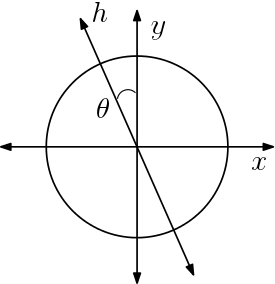
\includegraphics[width=.25\textwidth]{hw1_fig1.png}
\end{figure}

\item Suppose we obtain $1/\theta$ (whcih is given to be an integer $\geq 2$) training samples ({\em i.e.}, samples from $\mathcal{D}$, along with their true labels). What is the probability that we find a point whose label is ``inconsistent'' with $h$? Can you bound this probability by a constant independent of $\theta$?

\item Give an example of a distribution $\mathcal{D}$ under which $h$ has risk zero.
\end{enumerate}

\item Suppose $A_{1}, A_{2}, \ldots, A_{n}$ are events in a probability space.

\begin{enumerate}
\item Suppose $\Pr{A_{i}} = \frac{1}{2n}$ for all $i$. Then, show that the probability that none of the $A_{i}$'s occur is at least $1/2$.

\item Give a concrete example of events $A_{i}$ for which $\Pr{A_{i}} = \frac{1}{n-1}$ for all $i$, and the probability that none of them occur is zero.

\item Suppose $n \geq 3$, and $\Pr{A_{i}} = \frac{1}{n-1}$, but the events are all {\em independent}. Show that the probability that none of them occur is $\geq 1/8$.
\end{enumerate}

\item In our proof of the no-free lunch theorem, we assumed the algorithm $A$ to be deterministic. Let us now see how to allow randomized algorithms. Let $A$ be a randomized map from set $X$ to set $Y$. Formally, this means that for every $x \in X$, $A(x)$ is a random variabl, that takes values in $Y$. Suppose $\abs{X} < c\abs{Y}$, for some constant $c < 1$. 

\begin{enumerate}
\item Show that there exists $y \in Y$ such that $\max_{x\in X}\Pr{A(x) = y} \leq c$.
\item Show that this implies that for any distribution $\mathcal{D}$ over $X$, $\text{Pr}_{x\sim \mathcal{D}}(A(x) = y) \leq c$.
\end{enumerate}

\item Recall that the VC dimension of a hypothesis class $\mathcal{H}$ is the size fo the largest set that it can ``shatter.''

\begin{enumerate}
\item Consider the task of classifying points on a 2D plane, and let $\mathcal{H}$ be the class of axis parallel rectangles (points inside the rectangle are ``$+$'' and the poitns outside are ``$-$''). Prove that the VC dimension of $\mathcal{H}$ is 4.

\item This time, let $\chi = \mathbb{R}^{d}\backslash \{0\}$ (origin excluded), and let $\mathcal{H}$ be the set of all hyperplanes through the origin (points on one side are ``$+$'' and the other side are ``$-$''). Prove that the VC dimension of $\mathcal{H}$ is $\leq d$.

{\em Hint:} Consider {\em any} set of $d + 1$ points. They need to be linearly dependent. Now, could it happen that $u$, $v$ are ``$+$'', but $\alpha u + \beta v$ is ``$-$'' for $\alpha,\ \beta\geq 0$? Can you generalize this?

\item {\bf (BONUS)} Let $\chi$ be the points on the real line, and let $\mathcal{H}$ be the class of hypotheses of the form $\sign{p(x)}$, where $p(x)$ is a polynomial of degree at most $d$ (for convenience, define $\sign{0} = +1$). Prove that the VC dimension of this class is $d+1$. 

{\em Hint:} The tricky part is the uppoer bound. Here, suppose $d = 2$, and suppose we consider any four points $x_{1} < x_{2} < x_{3} < x_{4}$. Can the sign pattern $+$, $-$, $+$, $-$ arise from a degree 2 polynomial?
\end{enumerate}

\item In the examples above (and in general), a good rule of thumb for VC dimension of a function class is the {\em number of parameters} involved in defining a function in that class. However, this is not universally true, as illustrated in this problem: Let $\chi$ be the points on the real line, and define $\mathcal{H}$ to be the class of functions of the form $h_{\theta} \coloneqq \sign{\sin(\theta x)}$, for $\theta \in \mathbb{R}$. Note that each hypothesis is defined by the single parameter $\theta$.

Prove that the VC dimension of $\mathcal{H}$ is infinity.

So where does the ``complexity'' of the function class come from? {\bf (BONUS)} Prove that if we restrict $\theta$ to be a rational number whose numerator and denominator have at most $n$ bits, then the VC dimension is $\BigO{n}$.
\end{enumerate}
 
\end{document}